% Chapter 6

\chapter{Propuesta: Sistema Pytos} % Main chapter title

\label{ch:Chapter5} % For referencing the chapter elsewhere, use \ref{Chapter1} 

\lhead{Capítulo 5. \emph{Arquitectura de Pytos}} % This is for the header on each page - perhaps a shortened title

%----------------------------------------------------------------------------------------

En este capítulo son descritos los niveles jerárquicos involucrados en la Arquitectura de Pytos, a fin de realizar cómputo al borde de la red y 
optimizar los recursos móviles. 

\section{Arquitectura de Pytos}
\label{sec:pytosSystem}
Pytos es un \textit{framework} basado en Python que será implementado sobre un entorno \textit{cloudlet} con soporte de la nube. 
En la figura \ref{fig:pytosOverview} se muestran los componentes de Pytos desplegados sobre tres capas jerárquicas: (i) dispositivo cliente, 
(ii) \textit{cloudlet} y (iii) servidor 
en nube. La arquitectura propuesta cuenta con un componente privado, el cual es alojado y administrado en servidores de nuestro grupo 
de investigación. 
Este componente da soporte en el proceso de
descubrimiento de \emph{cloudlets} disponibles en una determinada red de área local. Los propósitos principales de que los servidores 
de consulta de \emph{cloudlets}
sean centralizados, en nube y administrados por Pytos; son: (i) seguridad, los programadores que usan Pytos pueden confiar su código en los cloudlets 
certificados por Pytos, (ii) disponibilidad, los \emph{cloudlet} disponibles en una red son consultados al servidor central de Pytos usando 
Internet desde cualquier lugar, y iii) facilidad, el desarrollador no se preocupa en instalar o desplegar el componente \emph{cloudlet}
. Entonces, el procedimiento mencionado de \emph{offloading} será realizado de forma transparente al usuario final y 
con facilidad para el desarrollador. Además de los beneficios en ahorro de energía y tiempo de respuesta en los móviles, consideramos 
una contribución importante la migración de tareas con envío a la nube, la cual se muestra en la parte a) de la Figura \ref{fig:pytosOverview}. 
A diferencia de la migración de tareas con data de retorno (donde las aplicaciones cliente están a la espera de un resultado desde el cloudlet
imagen b) de la Figura~\ref{fig:pytosOverview}), las aplicaciones con envío directo a nube entregan los resultados a una aplicación en nube 
especificada por el programador. Este modelo es útil cuando se realiza un pre-procesamiento antes de realizar \emph{streaming} de datos sin
necesidad
de volver al dispositivo móvil (codificación de video y audio, procesado de imágenes en tiempo real, etc.). En el caso no esté disponible   

%Esta arquitectura propuesta permite a las aplicaciones aliviar las limitaciones de los recursos móviles al migrar las tareas que 
%requieren un
%cálculo intensivo al \textit{cloudlet}. 


%desarrollador. El servidor de la nube de Pytos contiene un
%repositorio de \textit{cloudlets} disponibles por ubicación. Por lo tanto, se da libertad a los clientes consultar por el \textit{cloudlet}
%más cercano actualmente anexo a la red WLAN, a través de un proceso de descubrimiento de \textit{cloudlets}. Después de que Pytos es desplegado
%sobre los 3 niveles jerárquicos, Pytos decide si es ventajoso realizar \textit{offloading} al \textit{cloudlet} o no. 

El principal objetivo de la arquitectura propuesta es mejorar el rendimiento de los servicios basados en \textit{cloudlets} en lugares públicos 
de gran afluencia, como hospitales, restaurantes, cafetería o centros comerciales. Además, a través de la localización de \textit{cloudlets}, el 
framework puede facilitar y mejorar el rendimiento de aplicaciones que demanden gran cantidad de recursos, sensibles a la demora, trayendo los
recursos de la nube más cerca al usuario final.

\begin{figure}
\centering
 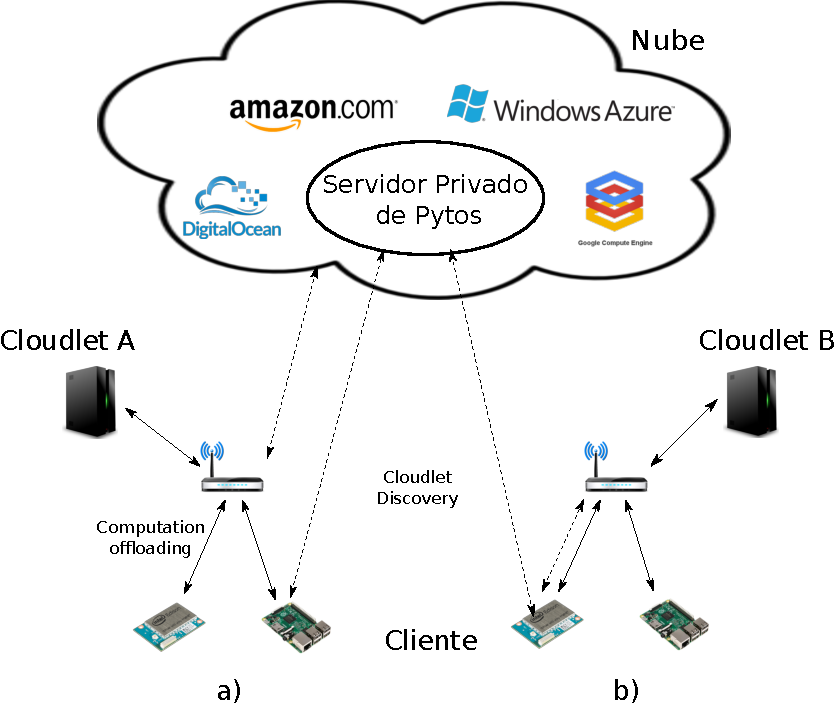
\includegraphics[scale=0.72]{Figures/generalArchitecture.pdf}
 \caption{Vista global de la arquitectura propuesta de Pytos}
 \label{fig:pytosOverview}
\end{figure}

Se propone un entorno de programación donde los desarrolladores seleccionen los métodos deseados de una aplicación que podrían ser migrados para
su ejecución remota. Cada vez que un método sea invocado y el servidor remoto esté disponible, Pytos usará su framework de optimización para decidir 
si el método debe ser migrado en tiempo de ejecución.
Con el objetivo de maximizar los beneficios de la infraestructura \textit{cloudlet}, se considera los siguientes componentes (ilustrados en la 
figura \ref{fig:pytosArchitecture}) : 

\begin{enumerate}
 \item \textbf{Biblioteca de Pytos:} Este componente provee la sintaxis para usar los decoradores de Pytos (descrito en la sección~\ref{sec:programmingModel}), el cual es precisado para interceptar
 el método de cómputo elevado. Además, inicializará un proceso demonio \textit{Pytos Daemon} si no ha sido inicializado uno anteriormente.
 \item \textbf{Pytos Daemon:} Es el componente fundamental del sistema de Pytos, el cual es compuesto de tres módulos principalmente:
 \begin{itemize}
\item El recopilador, que recauda información del contexto del móvil como: el estado de la red inalámbrica y el tiempo de ejecución en el servidor 
y el \textit{cloudlet}. Seguidamente, los valores del recopilador son enviados a la función de costo;
\item El evaluador o planificador de tareas, es responsable de evaluar la función de costo, ya que toma la decisión de \textit{offloading} más adecuada; y 
\item El explorador,  destinado a buscar nuevos \textit{cloudlets} disponibles. Como fue discutido anteriormente, este módulo consulta el repositorio
de \textit{cloudlets} de la aplicación localizados en el servidor en nube. 

\end{itemize}
 \item \textbf{Modelo de predicción:} En este componente se aborda el medio para optimizar la decisión de \textit{offloading}. En esta escena,
 un modelo probabilístico de regresión lineal es implementado para pronosticar el tiempo de ejecución de un método migrado al lado del
 \textit{cloudlet}. Entonces, los valores estimados son retornados al evaluador como una entrada en la función de costo.
 \item \textbf{\textit{Endpoints}\footnote{\url{https://cloud.google.com/appengine/docs/java/endpoints/}, Último acceso en setiembre 2015} de descubrimiento:} Ubicados en el componente \textit{cloudlet} donde una Interface de entrada en un Servidor
 Web (Web Server Gateway Interface, WSGI) \footnote{\url{https://www.python.org/dev/peps/pep-0333/}, último acceso en junio 2015} se ejecuta con la intención de dar soporte al cliente en el proceso de descubrimiento
 de \textit{cloudlets}. Se aprovecha el recurso centralizado en la nube para almacenar un repositorio general de \textit{cloudlets}.
 \item \textbf{Contenedor Pytos:} En este componente se ejecutará la tarea migrada de la aplicación. La función decorada definida 
 en el 
 código de programa inicial es convertida a \textit{endpoints} abiertos y accesible con un token de autorización basado en el modelo 
 distribuido REST. Los resultados son enviados nuevamente al cliente, o enviados directamente a la aplicación en nube especificada por el 
 desarrollador. Cada tarea migrada al poseer un \emph{token} único se podrá almacenar y utilizar nuevamente si es requerida por un periodo de tiempo.
 Los \textit{endpoints} son declarados usando un Identificador de Recurso Único (URI, Uniform Resource Identifier)~\cite{Walsh_architectureof}.
 \item \textbf{Aplicación web del Desarrollador:} Este componente es opcional. Si el desarrollador lo determinó en su aplicación cliente, el resultado 
 será enviado desde el contenedor Pytos hasta el servidor definido por el desarrollador. Por ejemplo, puede ser implementado un juego cooperativo 
 de realidad aumentada, el cual requiera procesar a cada frame de video antes de ser enviado a Internet. Creemos que tal proceso aliviaría 
 el costo operacional de los servidores en nube, delegando la tarea pesado de procesamiento de los frames a los \emph{cloudlets}. 
 
\end{enumerate}
En las secciones siguientes se describen los componentes indicados anteriormente en mayor detalle.

\begin{figure}
\centering
 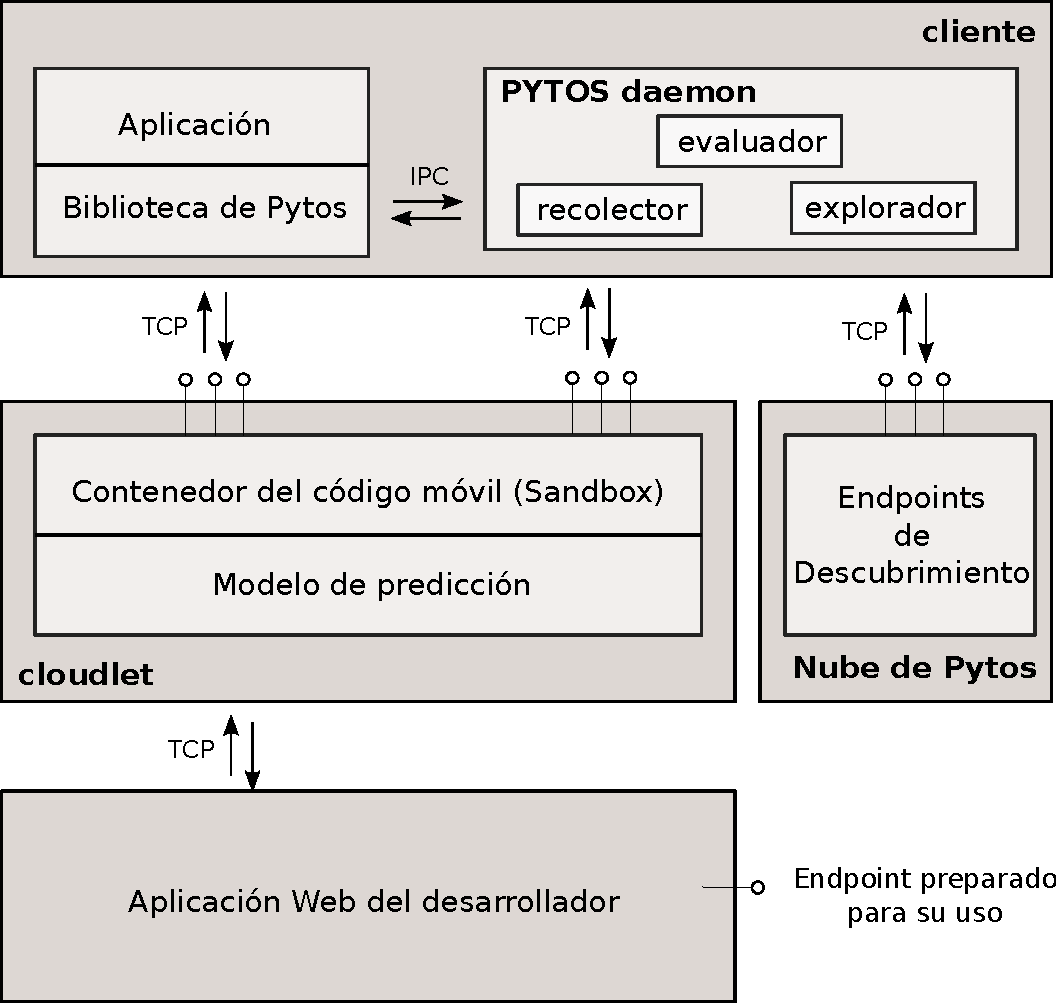
\includegraphics[scale=0.55]{Figures/components.pdf}
 \caption{Detalles de interacción entre los componentes de Pytos}
 \label{fig:pytosArchitecture}
\end{figure}


%%%%%%%%%%%%%%%%%%%%%%%%%%%%%%%%%%%%%%%%%%%%%%%%%%%%%%%%%%%%%%%%%%%%%%%%%%%%%%%%%%%%%%%%%%%%%%%%%%%%%%%
\section{Diseño de Pytos}
\label{sec:pytosDesign}
Después de la introducción inicial de las ventajas de migración de cómputo en el capítulo  \ref{ch:Chapter4} como una técnica para mejorar 
el rendimiento y reducir el uso de la batería en aplicaciones con cálculos intensivos; en esta sección son descritos los detalles de diseño
sobre la adición de la técnica de \textit{offloading} a una aplicación de una manera simple sin un esfuerzo adicional. Nuestro enfoque
tiene como objetivo la simplicidad, considerando:

\begin{enumerate}
 \item El uso de Python \footnote{\url{https://www.python.org/}, último acceso en junio 2015}, este lenguaje de programación de alto nivel es ampliamente usado para propósitos generales y tiene 
 una gran variedad de bibliotecas, las cuales en su gran mayoría son actualizadas periódicamente. 
 \item El uso de los \textit{decoradores} de Python \footnote{\url{https://www.python.org/dev/peps/pep-0318/}, último acceso en junio 2015}, 
 pues permite la selección a nivel de métodos. Tal cualidad permite 
 a los desarrolladores agregar \textit{offloading} de una manera sencilla.
 \item El proceso de descubrimiento de \textit{cloudlets} simple y transparente al usuario final
\end{enumerate}

\section{Modelo de Programación}
\label{sec:programmingModel}
Python tiene un modelo de programación potente, con características avanzadas y sintaxis expresiva. Uno de ellos son los \textit{decoradores},
los cuales generalmente son usados para alterar dinámicamente la funcionalidad de un método sin tener que usar directamente el uso de subclases. 
Esta característica encaja adecuadamente en nuestro enfoque para extender la funcionalidad de un método que \textit{puede} ser migrado fácilmente.
En el código \ref{list:pytosSample} se ilustra como un método es \textit{decorado} con la sintaxis de Pytos. Por lo tanto, el motor de Pytos podrá 
decidir en tiempo de ejecución si el \textit{offloading} es ventajoso o no.
%\vspace{0.5cm}

\begin{lstlisting}[caption= Ejemplo del uso de la sintaxis de Pytos sobre un método que \textit{puede} ser migrado, label=list:pytosSample]
@offload
def faceRecognition(self,img):
    faces = faceCascade.detectMultiScale(img,CTE1, CTE2)
    return faces
\end{lstlisting}

\vspace{0.5cm}
Luego que las funciones son seleccionadas, lo que el motor de Pytos hace es : 1) interceptará el código del método, 2) generar un código único o
\emph{token} que identifique al método, 3) encolar la tarea en el planificador inmediatamente, 4) revisar si es viable el envío de código al 
\emph{cloudlet}. 5) instalar el código de la función en el \emph{cloudlet} si es necesario, 6) ejecutar la tarea (local o remotamente) y esperar por 
el resultado (si no existe soporte de la nube). Las funciones \textit{decoradas} serán convertidas en puntos de salida HTTP
o \textit{endpoints} de la aplicación en el \textit{cloudlet} con identificadores URIs \footnote{\url{http://www.ltg.ed.ac.uk/~ht/WhatAreURIs/}}.


\subsection{Flujo del Sistema}
\label{sec:pytosWorkflow}
Nuestra propuesta de framework llevará a las aplicaciones móviles basadas en \textit{cloudlets} por los siguientes pasos antes de realziar la migración
de computación al \textit{cloudlet}. En la Figura ~\ref{fig:pytosWorkflow} se muestra el proceso de \textit{offloading} de cómputo.

\begin{enumerate}
 \item \textit{Proceso de descubrimiento de \textit{cloudlets}}: En esta fase, el explorador de Pytos solicita los \textit{cloudlets} disponibles
 en un red. Esta demanda toma el Identificador de Conjunto de Servicio\footnote{\url{http://www.webopedia.com/TERM/S/SSID.html}} (SSID, Service 
 Set Identifier) de la red WLAN que esté conectada en el momento como un parámetro de entrada.
 \item \textit{Decisión de \textit{offloading}:} Consecuentemente, en el siguiente paso es realizada la decisión inteligente de \textit{offloading}.
 En el cual el objetivo de Pytos es optimizar el rendimiento, por lo que el ancho de banda de la red y los tiempos de ejecución son 
 recolectados y transferidos a la función de evaluación (discutido en la sección~\ref{sec:intelligentOffloading})
 \item \textit{Ejecución de tareas pesadas}: La función de cómputo intensivo es ejecutada. Si es ejecutada remotamente, los parámetros del método
 y respuestas son colocados en una archivo con notación de Objeto JavaScript \footnote{\url{http://json.org/}, último acceso en febrero 2015}
 (JSON, JavaScript Object Notation). Entonces, estos datos
 livianos con enviados sobre la capa de transporte TCP.
\end{enumerate}

\begin{figure}
\centering
 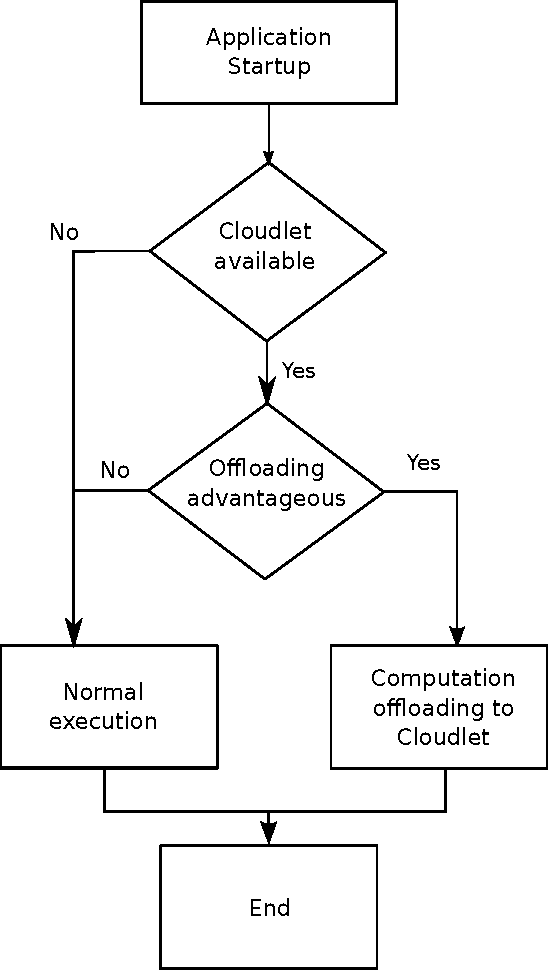
\includegraphics[scale=0.6]{Figures/pytosworkflow.pdf}
 \caption{Flujo del sistema de Pytos}
 \label{fig:pytosWorkflow}
\end{figure}


\section{Implementation}
\label{sec:implementation}

En esta sección resaltamos los detalles de implementación del framework Pytos. Se describe como el recopilador de red recolecta la información 
relevante del contexto móvil con el objetivo de realizar un \textit{offloading} inteligente antes de enviar el cómputo al \textit{cloudlet}. 
Finalmente, explicamos como el costo de evaluación es realizado priorizando el aspecto del rendimiento. 

%Finally, we show the architecture
%details of the components involved in our framework. 

\subsection{Recopilador}

Como mencionamos anteriormente, Pytos será capaz de realizar una decisión de \textit{offloading} inteligente en tiempo de ejecución: si la 
ejecución de la función debe ejecutarse remotamente o localmente. Para alcanzar tal objetivo, se implementará un recopilador a fin de recolectar
toda la información importante del contexto móvil, como: 1) características de la Red WLAN (ratio de transferencia, latencia) y 2) características
del contexto de la aplicación relacionadas al tiempo de ejecución en el \textit{cloudlet} y localmente (dispositivo móvil).

Para reunir el estado de la red, nosotros consideramos la técnica usada por Cuervo {\em et. al.}~\cite{Cuervo:2010:MMS:1814433.1814441}. Se 
implementará un proceso demonio de Pytos para enviar un paquete de 10kb al cloudlet a fin de medir el tiempo de transferencia. Usando este simple
enfoque permite que el recolector de Pytos obtenga los valores estimados de la latencia y ancho de banda. Tal procedimiento es realizado cada tres 
minutos para mantener un valor estimado actualizado. 
Similarmente, el proceso demonio de Pytos consulta el \textit{cloudlet} por información estadística basados en históricos sobre las funciones de 
cómputo pesado que fueron realizadas en el pasado. Luego, tales valores (1) y (2) son enviados a la función de costo (discutido en la Sección 
~\ref{sec:intelligentOffloading})

\subsection{Evaluador}
\label{sec:intelligentOffloading}
%The Pytos solver performs the cost function evaluation, using the information collected by Pytos profiler. 

Nuestra investigación se centra en minimizar el tiempo de ejecución de una función de cómputo pesado. En tal sentido, se construirá una función
de evaluación que considere lo siguiente: tiempo de ejecución en el \textit{cloudlet} y en el cliente, además del tiempo de transferencia. 
Estos valores son obtenidos del componente recopilador de Pytos. Usaremos la ecuación~\ref{eq:executiontimeFinal} explicada en la sección 
\ref{ch:Chapter4} como función evaluadora. 


%%%%%%%%%%%%%%%%%%%%%%%%%%%%%%%%%%%%%%%%%%%%%%%%%%%%%%%%%%%%%%%%%%%%%%%%%%%%%%%%%%%%%%%%%%%%%%%%%%%%%%%
\section{Resultados Iniciales}
\label{sec:evaluation}
En esta sección describimos la configuración experimental adoptada para evaluar la migración de tareas en un entorno \textit{cloudlet}. 
Dicho experimento en que factor el \textit{offloading} de cómputo es posible ahorrar energía y mejorar el rendimiento. Por lo que, se implementó
una aplicación de reconocimiento de rostros usando \textit{offloading} y fue probado sobre un conjunto de imágenes.


\subsection{Configuración experimental}

Con el objetivo de demostrar las ventajas del \textit{offloading} en un entorno \textit{cloudlet}, se consideraron los componentes de una 
jerarquía de tres niveles: cliente, \textit{cloudlet} y nube.

En el cliente, se utilizó una mini-computadora Intel Edison que incorpora la placa de expansión de Arduino 
\footnote{\url{https://www-ssl.intel.com/content/www/us/en/do-it-yourself/edison.html}, Último acceso en setiembre 2015} para direccionar la 
conexión con interfaces de Entrada/Salida externas como dispositivos de cámara web USB, tarjeta de expansión de memoria micro SD y entrada 
de energía. Esta placa incorpora un CPU Intel Atom con una frecuencia de 500 MHz de doble núcleo, 1 GB de memoria RAM y una antena WiFi 
interna IEEE 802.11a/b/g/n. 

Se usó como sistema operativo Ubilinux \footnote{\url{http://www.emutexlabs.com/ubilinux}, último acceso en setiembre 2015} 
de la distribución Debian (versión 150309). En el \textit{cloudlet} se utilizó una computadora de escritorio equipada con un CPU Intel Core i7-4700MQ
a una frecuencia de 2.40 GHz, 11.5 GiB de memoria RAM, y Ubuntu 14.04 como sistema operativo. En el servidor en nube se dispuso de una máquina 
virtual con Ubuntu 14.04 (7 núcleosy 16 GiB de memoria RAM), el cual pertenece a la empresa Digital Ocean~
\footnote{\url{https://www.digitalocean.com/}, último acceso en setiembre 2015} y está físicamente localizado en New York. 
Durante los ensayos, el ancho de banda de la conexión entre el cliente y el \textit{cloudlet}, medido con la herramienta Iperf benchmar 
\footnote{(\url{https://iperf.fr/}, último acceso en setiembre 2015}, fue aproximadamente 8.90 Mbits/seg. 
Todas las conexiones fueron realizadas sobre el protocolo TCP, usando un Punto de Acceso provisto por TP-link, en su modelo Archer C2.
Para obtener medidas de energía a grano fino, se consideró el uso de la herramienta PowerAPI~\cite{bourdon2013powerapi}, una biblioteca de 
software para monitorear la energía consumida a nivel de procesos. Dicha herramienta, nos permite conseguir de manera estándar y con alta precisión
(similar a los multímetros convencionales) las unidades \textit{watt} consumidas por el proceso deseado. Relegamos el consumo de energía realizado
por la interfase de WiFi, ya que este valor es dominado por el consumo de energía del CPU \cite{chen2015smartphone}. 

La metodología usada para obtener la energía y tiempo de respuesta se muestra en la Figura \ref{fig:experimentalSetup}. En tal procedimiento, 
el recopilador de datos, que está compuesto por el PowerAPI y un colector de marcas de tiempo, requiere el identificador de proceso o PID de la 
aplicación que implementa \textit{offloading} con Pytos. 

Antes de que se ejecute el \textit{offloading} de una aplicación, tal aplicación se detiene hasta que una señal de aviso del recopilador de datos
es recibida. Entonces, la aplicación que implementa Pytos comienza la tarea de cómputo pesado; simultáneamente, el consumo de energía y tiempo son 
recolectados para ser exportados. 

\begin{figure}[h]
\centering
 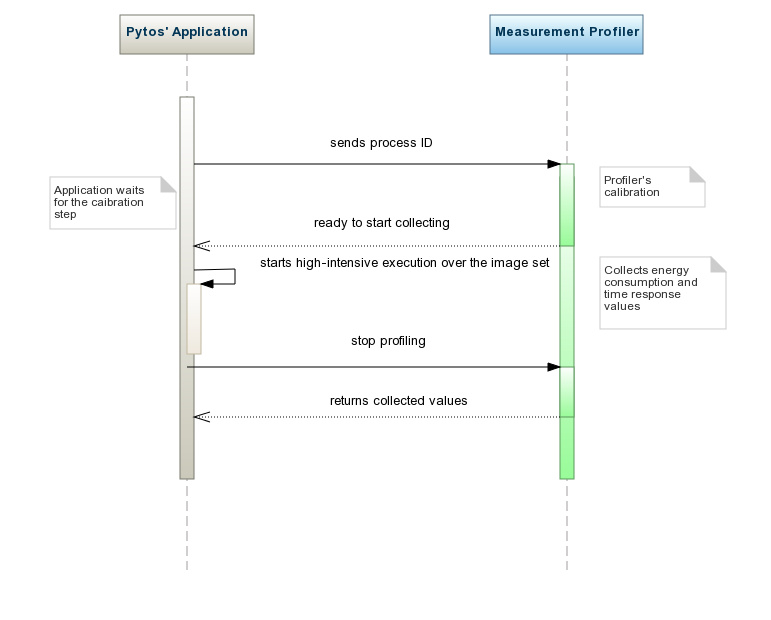
\includegraphics[scale=0.45]{Figures/experimentalEnvironment.jpg}
 \caption{Metodología para la medición}
 \label{fig:experimentalSetup}
\end{figure}

%\subsection{Application Sample}
\subsection{Escenarios de Evaluación}
\label{subsec:appsample}
Evaluamos la migración de tareas pesadas usando una aplicación de reconocimiento de rostros. Como mencionamos anteriormente, los desarrolladores 
deberán seleccionar en fase de diseño, los métodos costosos computacionalmente. Claramente, en este caso la operación que más necesita de recursos
es la de reconocimiento de rostros. De tal forma, si el cómputo es enviado a un \textit{cloudlet}, la aplicación principal espera por la respuesta
a fin de ser mostrado en el dispositivo limitado. 
En el cuadro~\ref{table:imageSet} se muestra el conjunto de imágenes que fueron probados con nuestra aplicación. Cada conjunto contiene 20 
imágenes que fueron obtenidas de una misma cámara web. 

\begin{table}[]
\centering
\caption{Datos de los diferentes conjuntos de imágenes usados en la aplicación de reconocimiento de rostros}
\label{table:imageSet}
\begin{tabular}{|c|c|c|c|}
\hline
{\bf Set} & {\bf \begin{tabular}[c]{@{}c@{}}Resolution\\ (width x height)\end{tabular}} & {\bf \begin{tabular}[c]{@{}c@{}} Average size  \\ (bytes)\end{tabular}} & {\bf \begin{tabular}[c]{@{}c@{}} Standard  \\ deviation \end{tabular}} \\ \hline
1         & 160x120                                                                     & 7612                                                          & 141                                                                         \\ \hline
2         & 176x144                                                                     & 8959                                                          & 203                                                                         \\ \hline
3         & 416x240                                                                     & 21478                                                         & 1183                                                                        \\ \hline
4         & 352x288                                                                     & 23548                                                         & 1494                                                                        \\ \hline
5         & 800x600                                                                     & 84668                                                         & 810                                                                         \\ \hline
6         & 960x544                                                                     & 89023                                                         & 5098                                                                        \\ \hline
\end{tabular}
\end{table}

\subsection{Resultados Iniciales}



\begin{figure}
\centering
 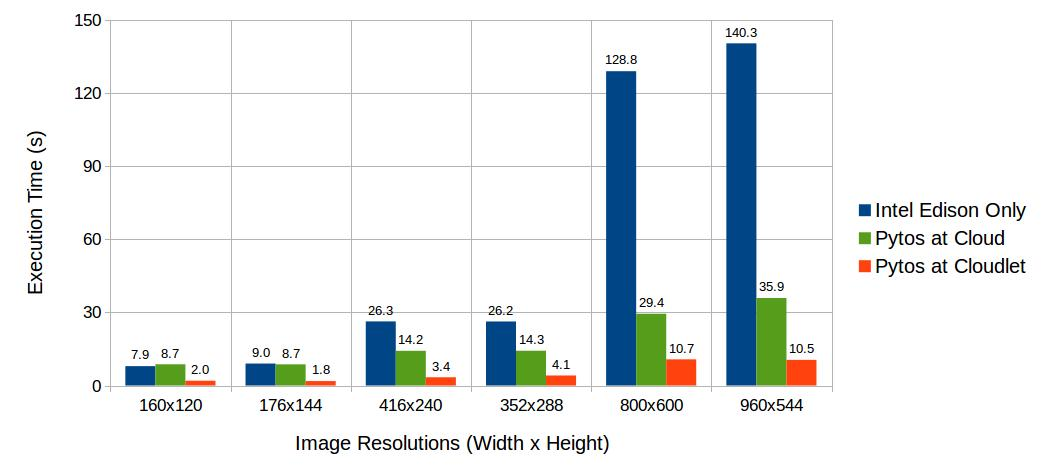
\includegraphics[scale=0.35]{Figures/timeRepsonseBenchmark}
 \caption{Comparación de tiempo de respuestas usando diferentes escenarios.}
 \label{fig:timesResponseBenchmark}
\end{figure}

\begin{figure}
\centering
 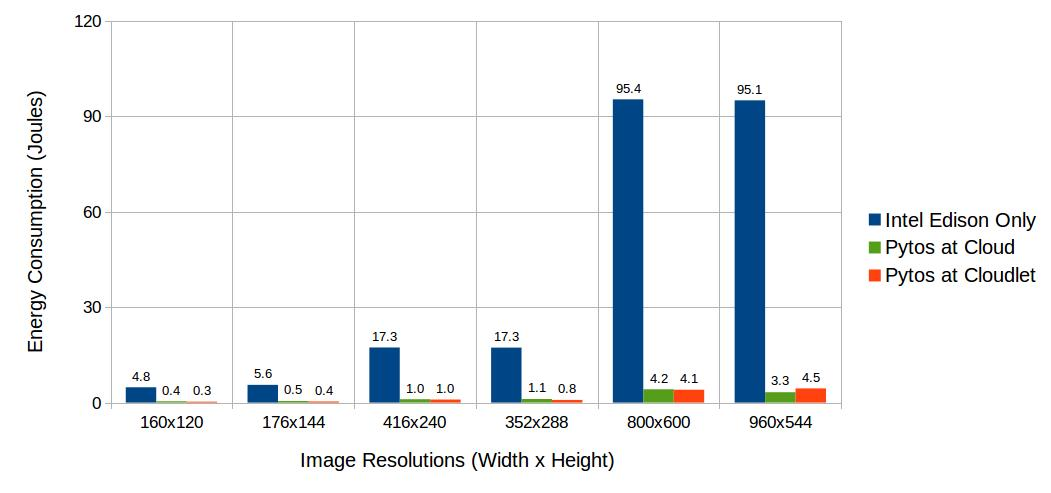
\includegraphics[scale=0.35]{Figures/energyBenchmark}
 \caption{Comparación de energía consumida usando diferentes escenarios.}
 \label{fig:energyBenchmark}
\end{figure}
%modified
Se evaluó localmente (cliente) y remotamente (\textit{cloudlet} y nube) el rendimiento y el ahorro de energía de una aplicación que usualmente consume abundantes recursos (descrito en 
la Sección~\ref{subsec:appsample}). Los experimentos son ejecutados en tres escenarios: (1)solamente en el dispositivo Intel Edison (2)
en la infraestructura \textit{cloudlet}, y (3) sobre la infraestructura en nube. El último escenario no es un objetivo del framework propuesto,
sin embargo, lo consideramos para notar el impacto de la demora en los escenarios WAN. 

La Figura~\ref{subsec:appsample} muestra la diferencia de rendimiento al procesar los conjuntos (1), (2) y (3) de las
imágenes variables (Cuadro \ref{table:imageSet}). Como se esperaba, a medida que la imagen de entrada a ser procesada era más grande, más tiempo
se requería para su procesamiento; en todos los escenarios. Por ejemplo, para la ejecución aislada en Intel Edison varía desde 7.94 segundos (s)
(con una desviación estándar de  0.0215) para procesar el conjunto 1 de imágenes más liviano a 140 s (con una desviación estándar de 0.2571)
para procesar el conjunto más pesado. Mientras tanto, empleando la infraestructura \textit{cloudlet} se utilizó 1.98 s (con una desviación estándar de
0.4839) para procesar el conjunto 1, y 10.53 s para procesar el conjunto 6, eso significa que el rendimiento se acrecentó en un factor de
4 a 13 veces. Los experimentos usando la nube muestran un rendimiento bueno en comparación con la ejecución aislada en Intel Edison, pero son peores
en comparación con los ejecutados en entornos \textit{cloudlets} debido a la latencia WAN elevada. Por lo que se confirma que la ejecución de 
tareas pesadas en \textit{cloudlets} es una mejor apuesta.

Similarmente, la Figura~\ref{fig:energyBenchmark} muestra la misma tendencia en ahorro de energía. La energía en ejecución aislada en 
Intel Edison varía desde 4.81 Joules (J) (con una desviación estándar de 0.0822) para procesar el conjunto 1, a 95.06 J
(con una desviación estándar de 0.3077) para procesar el último conjunto de imágenes 6. Por otra parte, migrando cómputo al \textit{cloudlet}
varía de  0.29 J (con una desviación estándar de 0.0217) para procesar el conjunto 1 (economizando energía en un factor de 16), a 4,45 J (desviación
estándar de 0.1884) para procesar el conjunto 6 (economizando energía en un factor de 21).

